\documentclass[11pt]{article}

\usepackage{graphicx}
\usepackage{color}
\usepackage{algorithm}
\usepackage{algpseudocode}

\usepackage[T1]{fontenc}
\usepackage[utf8]{inputenc}
\usepackage{indentfirst}
\usepackage{dsfont}

\usepackage[justification=centering]{caption}

\usepackage{amsmath}
\usepackage{amssymb}

\usepackage{multicol}
\usepackage{url}
\usepackage{siunitx}

\setlength{\parskip}{1em}

\title{HW2 $-$ Semiclassical quantization of molecular vibrations}
\author{Enrique Gómez Cruz\\Facultad de Ciencias, Universidad Nacional Autónoma de México.}
\date{}

\begin{document}
\maketitle

  
According to quantum mechanics, in a diatomic molecule such as $H_2$, there are just an integer number of allowed energies. In this project, a search of the quantized energy levels are going to be searched numerically using two different models of the potential that describes the binding of the nucleus.

We consider the dimensionless action at a given energy
\begin{equation*}
  S(E) = \oint k(r) dr,
\end{equation*}
where $k(r) = p(r)/\hbar$ is the local de Broglie wave number and 
\begin{equation*}
 p(r) = \pm[2m(E-V(r))]^{1/2}
\end{equation*}
is the momentum that, classically, describes the oscillation of the system between $r_{in}$ and $r_{out}$.

The quantization of the system is achieved by stating that the de Broglie wave number, $k(r)$, should be $(n+1/2)2 \pi$, with $n\in\mathds{N}$. This gives us
\begin{equation}
  S(E_n) = 2\int_{r_{in}}^{r_{out}}\left(\frac{2m}{\hbar^2}\right)^{1/2} \left[E_n-V(r)\right]^{1/2} dr = \left(n+\frac{1}{2}\right) 2\pi
\label{eqn:action}
\end{equation}

For the diatomic molecule, $H_2$, $\gamma = 21.7$ and $V_0 = \SI{4.747}{\volt}$. Also, experimentally, the quantized energies are
\begin{table}[H]
\centering
\caption{Quantized energies for the diatomic molecule $H_2$}
\label{tbl:energy}
\begin{tabular}{ll|ll}
$n$ & $E_n(\SI{}{\electronvolt})$  & $n$ & $E_n(\SI{}{\electronvolt})$  \\\hline
0   & -4.477 & 8   & -1.151 \\
1   & -3.962 & 9   & -0.867 \\
2   & -3.475 & 10  & -0.615 \\
3   & -3.017 & 11  & -0.400 \\
4   & -2.587 & 12  & -0.225 \\
5   & -2.185 & 13  & -0.094 \\
6   & -1.811 & 14  & -0.017 \\
7   & -1.466 &     &       
\end{tabular}
\end{table}

\subsection{Modelling with the Lennard-Jones potential}
\begin{equation*}
  V(r)= 4 V_0\left[\left(\frac{a}{r}\right)^{12}-\left(\frac{a}{r}\right)^{6}\right]
\end{equation*}
Given the Lennard-Jones potential we can define
\begin{equation*}
  \epsilon \equiv \frac{E}{V_0}\qquad x\equiv\frac{r}{a}\qquad \gamma \equiv \left(\frac{2ma^2V_0}{\hbar^2}\right)^{1/2}
\end{equation*}
and the scaled potential as
\begin{equation*}
  v(x)= 4\left(\frac{1}{x^{12}}-\frac{1}{x^6}\right)
\end{equation*}
to get
\begin{equation}
  s(\epsilon_n) = \gamma\int_{x_{in}}^{x_{out}} \left[\epsilon_n-v(x)\right]^{1/2} dx = \left(n+\frac{1}{2}\right)\pi
  \label{eqn:scaled_action}
\end{equation}
\begin{figure}[H]
  \centering
  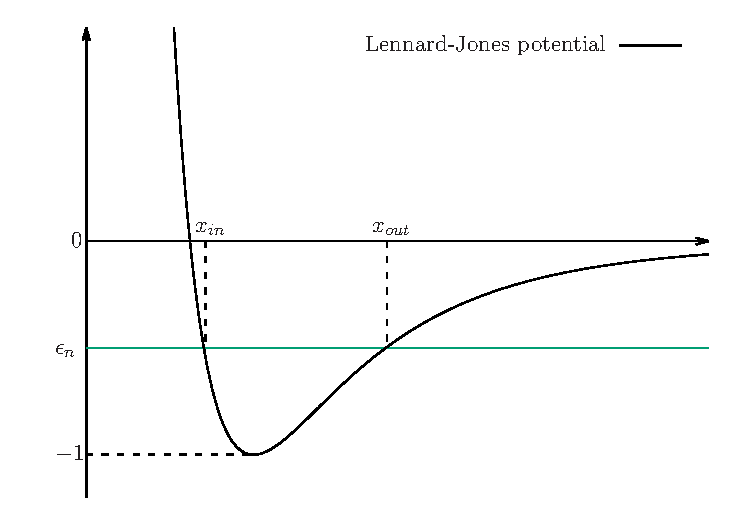
\includegraphics[width=.8\linewidth]{potential-LJ}
  \caption{Scaled Lennard-Jones potential}
\label{fig:potential-Lj}
\end{figure}
Analytically, $x_{in}$ and $x_{out}$ can be obtained by finding the roots of the equation $\epsilon-v(x) = 0$. This roots are
\begin{align*}
  x_{in} &= \sqrt[6]{\frac{2}{\epsilon}\left(-1+\sqrt{1+\epsilon}\right)}\\
  x_{out} &= \sqrt[6]{\frac{2}{\epsilon}\left(-1-\sqrt{1+\epsilon}\right)}
\end{align*}

Knowing $x_{in}$ and $x_{out}$, the integral in equation~\ref{eqn:scaled_action} can be calculated. Bode's rule was used to calculate the action, $s$, for each energy $\epsilon\in(-1,0)$.
\begin{figure}[H]
  \centering
  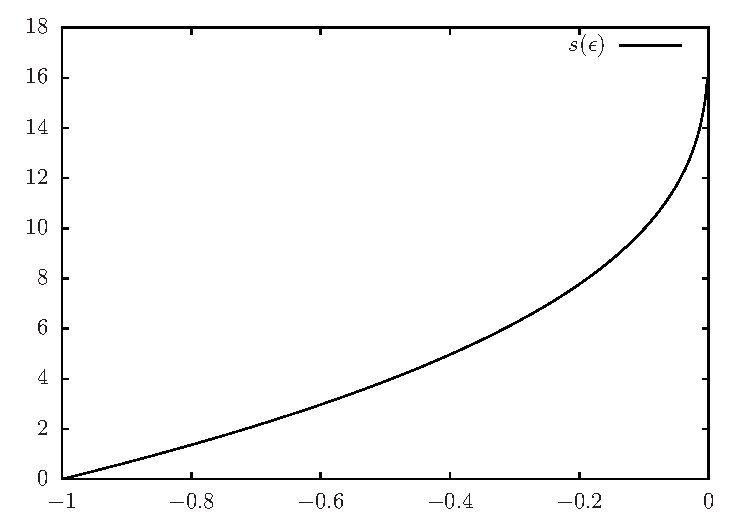
\includegraphics[width=\linewidth]{action-LJ}
  \caption{Action for each dimensionless energy $\epsilon$.}
\label{fig:action-Lj}
\end{figure}

And finally, with the quantization rule in the right hand side of equation~\ref{eqn:scaled_action} we can obtain the permitted energy levels by getting the roots of the function
\begin{equation*}
  f(\epsilon, n) = s(\epsilon) - \left(n+\frac{1}{2}\right)\pi
\end{equation*}
\begin{figure}[H]
  \centering
  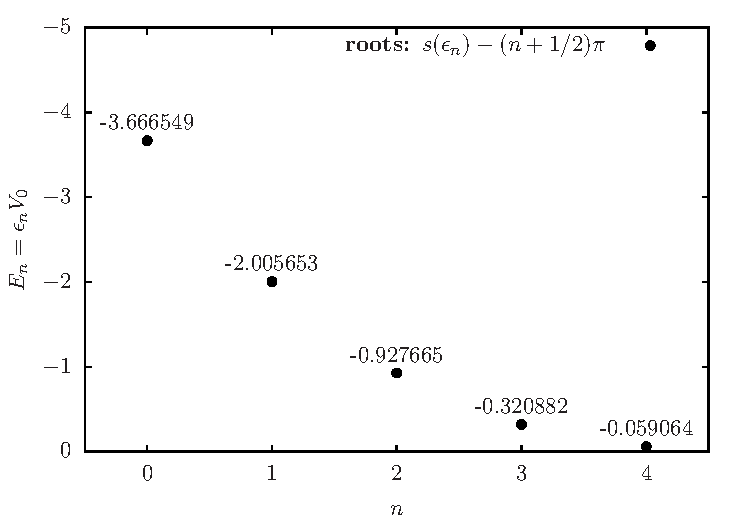
\includegraphics[width=\linewidth]{quantizedEnergy-LJ}
  \caption{Quantized energy levels $E_n$.}
\label{fig:energy-LJ}
\end{figure}

It can be seen, by comparing figure~\ref{fig:energy-LJ} with table~\ref{tbl:energy}, that we don't get exactly the energies that the experiment shows.

The Lennard-Jones model only predicts energies for $n\le5$. For bigger $n$ the energies diverge.

Numerically, energies where obtained until $n\le4$ because the algorithm implemented lacked precision. An implementation made using the GSL library did give all predicted energies.

\subsection{Modelling with the Morse potential}
\begin{equation*}
  V(r) = V_0\left[\left[1-\exp{\left(\frac{r_{min-r}}{\beta}\right)}\right]^2-1 \right]
\end{equation*}
\begin{figure}[H]
  \centering
  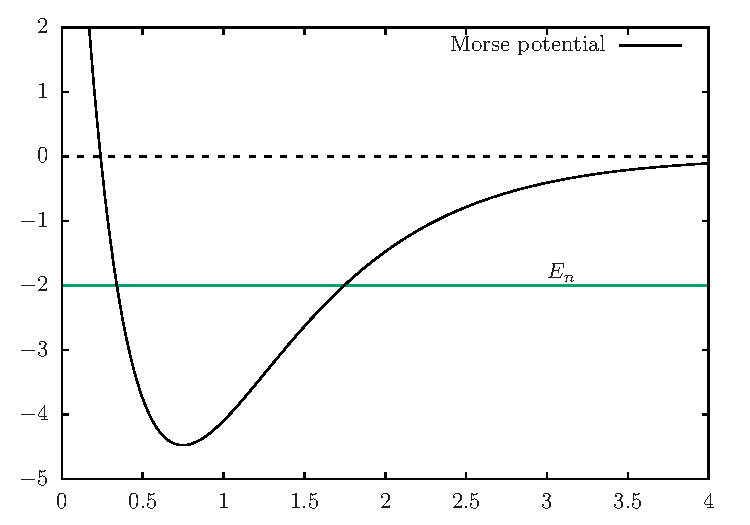
\includegraphics[width=\linewidth]{potential-Morse}
  \caption{Morse potential.}
\label{fig:potential-Morse}
\end{figure}
In this model $r_{min}$ is used to define the lowest point of the potential and $\beta$ is used to adjust the width of the potential. $r_{min}$ is experimentally known to be $\SI{0.74166}{\angstrom}$. $\beta$ was adjusted by trial and error to corrrectly give the known energies for $H_2$.

To integrate equation~\ref{eqn:action} we obtain, analytically, $r_{in}$ and $r_{out}$
\begin{align*}
  r_{in} &= r_{min} -\beta\log\left(1+\sqrt{\frac{E}{V_0}+1}\right)\\
  r_{out}&= r_{min} -\beta\log\left(1-\sqrt{\frac{E}{V_0}+1}\right)
\end{align*}
For each energy we integrate to obtain the action of the system.
\begin{figure}[H]
  \centering
  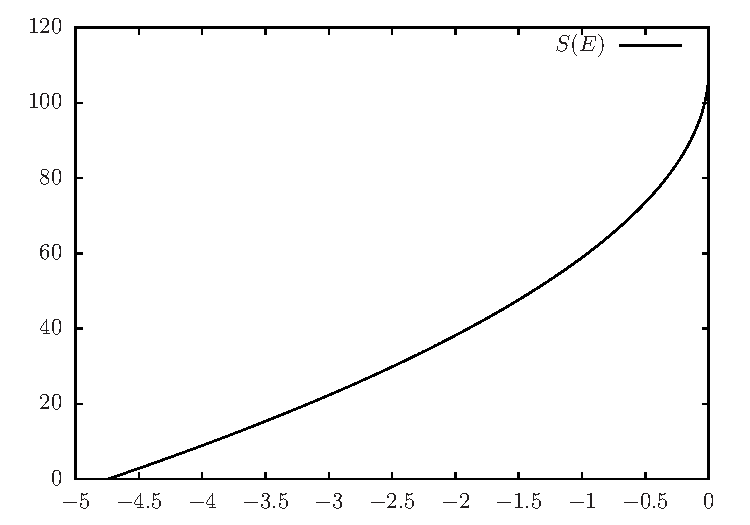
\includegraphics[width=\linewidth]{action-Morse}
  \caption{Action for each energy $E$.}
\label{fig:action-Morse}
\end{figure}
And the quantization restriction of equation~\ref{eqn:action} allows us to get the permitted energies for the system
\begin{figure}[H]
  \centering
  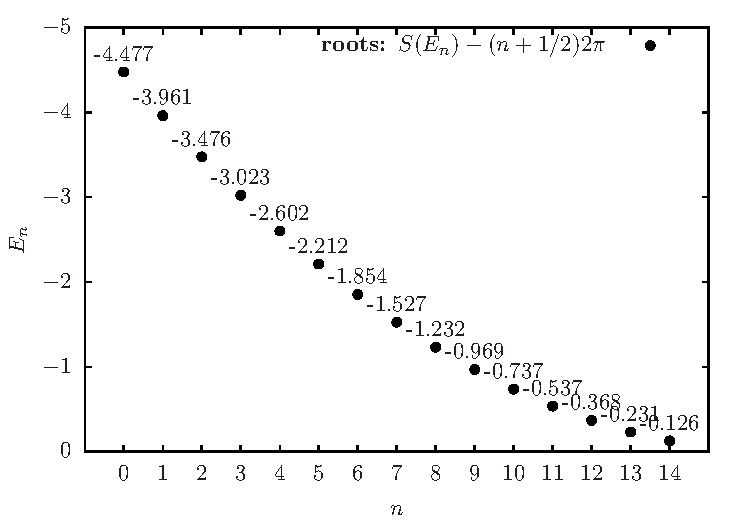
\includegraphics[width=\linewidth]{quantizedEnergy-Morse}
  \caption{Quantized energy levels $E_n$.}
\label{fig:energy-Morse}
\end{figure}

\end{document}
